	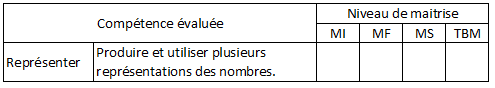
\includegraphics[scale=0.95]{competences}

\section{Calculer}
Calculer les expressions suivantes en détaillant tous les calculs:
\begin{questions}
	
	\question[1]  \'Ecrire en toutes lettres le nombre \num{5400125639.005}
	
	%\fillwithdottedlines{2cm}
	\begin{solution}
		cinq-milliards-quatre-cent-millions-cent-vingt-cinq-mille-six-cent-trente-neuf unités cinq-millièmes.
	\end{solution}
	
	
	\question[1]  \'Ecrire en chiffres le nombre cinq-cent-milliards-dix-millions-sept-cent-quarante-trois-mille unités deux-cent-soixante-quatre millièmes
	
	%\fillwithdottedlines{2cm}
	\begin{solution}
		\num{500010743000.264}
	\end{solution}
	
	\question[1]  \'Ecrire en chiffres le nombre cinquante-trois-milliards-huit-cent-un-millions-quarante-trois unités mille-deux-cent-vingt-cinq millièmes
	
	%\fillwithdottedlines{2cm}
	\begin{solution}
		\num{53801000044,225} ou \num{53801000043,1225} ou \num{53801000043,225} (erreur d'énoncé)
	\end{solution}
	
	\question[1]  Donner le nombre de dizaines de milliers de $\num{45753438254}$
	
	%\fillwithdottedlines{2cm}
	\begin{solution}
		Le nombre de dizaines de milliers est \num{4575343}.
	\end{solution}
	
	\question[1]  \'Ecrire en toutes lettres le nombre \num{4580125639.245}
	
	%fillwithdottedlines{2cm}
	
	\begin{solution}
		Quatre-milliards-cinq-cent-quatre-vingt-millions-cent-vingt-cinq-mille-six-cent-trente-neuf unités deux-cent-quarante-cinq millièmes.
	\end{solution}	
	
	
	\newpage
	
	\question[1]  Calculer $\num{45753438254} \times 1000$
	
	%\fillwithdottedlines{2cm}
	\begin{solution}
		$\num{45753438254} \times 1000 = \num{45753438254000}$
	\end{solution}
	
	\question[1]  Donner le chiffre des dizaines de milliers de $\num{45753438254}$
	
	%\fillwithdottedlines{2cm}
	\begin{solution}
		Le chiffre des dizaines de milliers est 3.
	\end{solution}
	
	
	
	
	
	\question[1]  Calculer $\num{38.254} \div 1000$
	
	\fillwithdottedlines{2cm}
	
	
	\question[1]  Calculer $\num{45753.438254} \times 100$
	
	\fillwithdottedlines{2cm}
	
	\question[1]  Calculer $\num{45753438254} \div 1000$
	
	\fillwithdottedlines{2cm}
\end{questions}


